
\documentclass[a4paper,10pt,fleqn]{article} % Definiert Papier = A4;
                                            % Schriftgrösse = 10Punkte;
                                            % Mathe.-Gl. Modus = linksbündig
                                            % (siehe http://lefti.amigager.de/latex/Aufbau.html)

\usepackage[utf8x]{inputenc}                % utf8x kann alle Textcodierungen interpretieren
\usepackage[T1]{fontenc} %Schriftcodierung mit UTF-8
\usepackage{textcomp} %Erweiterung von fontenc
\usepackage{lmodern} %Erweiterung des Zeichensatzes

\usepackage{graphics}                       % Package für Einfügen/Anpassen von Grafiken
\usepackage{graphicx}
\usepackage{wrapfig}                        % Package zum Einfügen von Textumflossenen Bilder

\usepackage[english,ngerman]{babel}         % ngerman = Neues Deutsch; babel = internationalisierung einschalten
\usepackage[babel,german=quotes]{csquotes}  % Deutsche Gänsefüssechen

\usepackage{hyperref}

\usepackage{amsmath}                        
\usepackage[all]{xy}
%\usepackage[xindy]{glossaries}
\usepackage{makeidx}
\usepackage{pdfpages}
\usepackage{graphicx}
\usepackage{printlen}

\usepackage{blindtext}
\usepackage{lipsum}

\usepackage{multicol}

\usepackage{multirow}

\usepackage{verbatim}

\usepackage{color}

\usepackage{eurosym}

%\usepackage{hyperref}
\usepackage{acronym}

\usepackage{enumitem}

\usepackage{setspace}

\usepackage{threeparttable} %benötigt um Fussnoten in einer Tabelle zu machen
\usepackage{longtable}


\usepackage{spreadtab} %benötigt um in Tabellen zu rechnen
\usepackage{numprint}

%Package damit eine Seite quer genommen werden kann
\usepackage{lscape}

%Damit man eine Zelle farbig markiert werden
\usepackage{colortbl}


%
% Rechnen in Tabellen. Zeichen für den Dezimalpunkt
%
\STsetdecimalsep{{.}}

\definecolor{darkgreen}{rgb}{0,0.6,0}
\usepackage{listings}
\lstset{language=[LaTeX]TeX}
\lstloadlanguages{TeX}
\lstset{basicstyle=\ttfamily\footnotesize,
        numbers=left,
        numberstyle=\tiny,
        numbersep=5pt,
        breaklines=true,
        texcsstyle=\color{black},
        backgroundcolor=\color{gray!10},
        %commentstyle=\color{darkgreen},
        %keywordstyle=\color{red}\bfseries,
        %stringstyle=\color{blue}\bfseries,
        frame=single,
        tabsize=2,
        rulecolor=\color{black!30},
        title=\lstname,
        escapeinside={\%*}{*)},
        breaklines=true,
        breakatwhitespace=true,
        framextopmargin=2pt,
        framexbottommargin=2pt,
        inputencoding=utf8x,
        extendedchars=true,
        literate={Ö}{{\"O}}1
                 {Ä}{{\"A}}1
                 {Ü}{{\"U}}1
                 {ü}{{\"u}}1
                 {ä}{{\"a}}1
                 {ö}{{\"o}}1 
       }
%
% hypersetup etwas genauer
%
\hypersetup{pdftex=true,
            hyperfigures=true,
            hyperindex=true,
            bookmarks=true,
            bookmarksopen=true,
            bookmarksnumbered=true,
            %pdfborder={0 0 0},
            hypertexnames=true,
            colorlinks=true,
            pagebackref=false,
            linktocpage=false,% link "`behing"'
            plainpages=false,
            linkcolor=black,%blue,
            %anchorcolor=black,% Color for anchor text.
            citecolor=black,%green,%Color for bibliographical citations in text.
            filecolor=black,%magenta,%Color for URLs which open local files.
            menucolor=black,%red,%Color for Acrobat menu items. pagecolor color red Color for links to other pages, but currently unused
            urlcolor=black,%red,
            pdfstartview=Fit,
            pdfview={XYZ null null null},
            pdfpagelabels,
            pageanchor=true,
            hypertexnames=false
           }
%
% hypersetup etwas rudimentärer
%
%{
    %colorlinks,
    %citecolor=black,
    %filecolor=black,
    %linkcolor=black,
    %urlcolor=black
%}

\usepackage{url}

\usepackage{cite}
\usepackage{apacite}

\usepackage{pdfpages}                        % Packet für PDF Dateimanipulation laden

\usepackage{fancyhdr}                        % http://en.wikibooks.org/wiki/LaTeX/Page_Layout#Customising_with_fancyhdr

\usepackage{siunitx}                         % benötigt um Tabellen nach einem . auszurichten


\bibliographystyle{apacite}


\pagestyle{fancy} %eigener Seitenstil
\fancyhf{} %alle Kopf- und Fusszeilenfelder bereinigen

\addtolength{\textwidth}{1.5cm}
\addtolength{\evensidemargin}{-5mm}
\addtolength{\oddsidemargin}{-5mm}

\addtolength{\headwidth}{1.5cm}

%\rhead{\setlength{\unitlength}{1mm}
%\begin{picture}(-2,7)
%    \includegraphics[width=35mm]{hslu_logo2.PNG}
%\end{picture}}

\fancyhead[L]{Projektarbeit: Autonomer Ballwerfer} %Kopfzeile links
\fancyhead[C]{} %zentrierte Kopfzeile
\fancyhead[R]{HSLU - T\&A}
%\fancyhead[R]{\includegraphics[scale=0.25]{hslu_logo2.PNG}}
\renewcommand{\headrulewidth}{0.4pt} % obere Trennlinie
\fancyfoot[L]{PREN Team 32}
\fancyfoot[C]{HS - 2014}
\fancyfoot[R]{\thepage}
\renewcommand{\footrulewidth}{0.4pt} % untere Trennlinie

%
% Anpassung der Darstellung des Literaturverzeichnis
%
\let\oldbibliography\thebibliography
\renewcommand{\thebibliography}[1]{%
  \oldbibliography{#1}%
  \setlength{\itemsep}{10pt}%
}
%
% Abbildungen und Tabellen nur mit Kurzform angeben
%
\addto\captionsngerman{
\renewcommand{\figurename}{Abb.}
\renewcommand{\tablename}{Tab.}
}
%
% Benötigt um von zwei Stellen im Text auf dieselbe Fusszeile zu referenzieren
%
\newcommand{\footnoteremember}[2]{%
  \footnote{#2\label{#1}}
  \newcounter{#1}
  \setcounter{#1}{\value{footnote}}
}
\newcommand{\footnoterecall}[1]{%
  \hyperref[#1]{\footnotemark[\value{#1}]}
} 
\makeatletter
\providecommand{\rowno}[1][__empty__]
{%
  \ifthenelse{\isundefined{\c@rowno}}
  {%
    \newcounter{rowno}
  }
  {}%
  	\ifthenelse{\equal{#1}{__empty__}}
 	 {%
       \stepcounter{rowno}%
     }
     {%
 	   \setcounter{rowno}{#1}%
     }%
  \therowno%
}
\makeatother
%
%\makeglossaries
%\include{wa/wa_glossar}
%
\newcommand{\myTitel}{Morphologischer Kasten}
\begin{document}
    %
    % Deck- und Titelblatt
    %
    \begin{titlepage}
    \begin{center}     
        \parindent0pt{\Huge PREN 1}\\
        \vspace*{1.2cm}
        Yves Studer\\
        Thomas Wiss\\
        Livio Kunz\\
        Nikolaus Manser\\
        MatteoTrachsel\\
        Güdel Manuel\\
        Pascal Roth\\
        \vspace*{1.2cm}
        {\Huge \myTitel}\\
        \vspace*{1cm}
%        \begin{figure*}[h!]
%            \centering
%            \includegraphics[width=0.7\textwidth]{Sourcen/Bilder/WuerfelTitel}
%        \end{figure*}
        \vspace*{10cm}
        {\normalsize Hochschule Luzern - Technik \& Architektur}\\
        {\normalsize PREN 1}\\
        \vspace*{0.6cm}
        {\normalsize Horw, Hochschule Luzern - T\&A, \today}\\
    \end{center}
\end{titlepage}

    \begin{titlepage}
    \parindent0pt {\Huge PREN 1}\\
    \vspace*{0.7cm}
    \newline
    \begin{tabular}{ p{6cm} p{5cm}}
        Yves Studer                & Thomas Wiss \\
        Dorfstrasse 28             & Bachhüsliweg 4a \\
        6264 Pfaffnau              & 6042 Dietwil \\
        +41 79 705 48 88           & +41 79 604 93 61 \\
        yves.studer@stud.hslu.ch   & thomas.wiss@stud.hslu.ch \\
                                   & \\
        Livio Kunz                 & Niklaus Manser \\
        Hubelmatt 7                 & Brunnmattstrasse 11\\
        6206 Neuenkirch         & 6010 Kriens \\
        +41 79 811 53 03           & +41 77 405 58 56 \\
        livio.kunz@stud.hslu.ch    & niklaus.manser@stud.hslu.ch \\
                                   & \\
        Matteo Trachsel			   & Manuel Güdel \\
        Hofstrasse 4               & Riedtalstrasse 4\\
        6004 Luzern                & 4800 Zofingen\\
        +41 79 511 57 88           & +41 79 774 41 40 \\
        matteo.trachsel@stud.hslu.ch & manuel.guedel@stud.hslu.ch \\
        						   & \\
        Pascal Roth			       & \\
        Dorfstrasse 18			   & \\
        6275 Ballwil		       & \\
        +41 79 717 68 94	       & \\
        pascal.roth@stud.hslu.ch   & \\
    \end{tabular}
    \vspace*{1.7cm}
    \newline
    {\Huge Meilenstein 1 Dokumentation}\\
    \vspace*{1.2cm}\\
    {\normalsize Dozent: Markus Thalmann}\\
    \vspace*{0.2cm}\\
    {\normalsize Hochschule Luzern - Technik \& Architektur}\\
    {\normalsize Interdisziplinäre Projekarbeit 2014}\\
    \vspace*{2.3cm}
    \newline
    {\normalsize Horw, Hochschule Luzern - T\&A, \today}\\
\end{titlepage}

    %
    % Inhlatsverzeichnis umbenennen und anschliessend einen Seitenumbruch
    % 
    \begin{tabular}{|p{1.2cm}|p{1.2cm}|p{6cm}|p{3cm}|} \hline
\textbf{Version} & \textbf{Datum} & \textbf{Änderung} & \textbf{Verantwortlicher}\\ \hline
v1.0 & 25.9.14 & Dokument erstellt & Yves Studer\\ \hline
 &  &   &  \\ \hline
 &  &   &  \\ \hline
\end{tabular}  
    \renewcommand{\contentsname}{Inhalt}
    \tableofcontents
    \newpage
    
    %
    % Start mit der eigentlichen Arbeit
    %  
    \section{Analyse}
	Als Gesamtübersicht und als Eruierungshilfe der einzelnen Teilprobleme haben wir zu Beginn der Lösungsfindung eine Skizze entworfen. Diese beinhaltet alle nötigen Elemente des Produkts und stellt diese in Relation zueinander dar. 
	
	\begin{figure}[h!]
		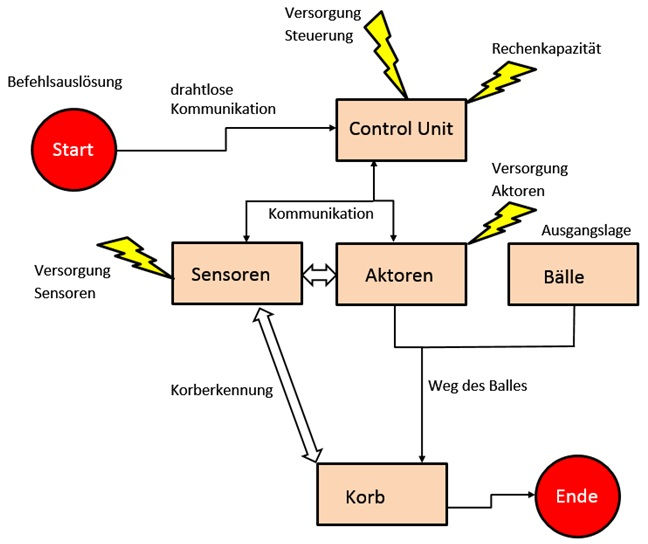
\includegraphics[width=0.9\textwidth]{Morphologie/Bilder/Blockschaltbild.jpg}
		\centering
		\caption{Funktionsskizze zur Aufgabenstellung}
		\label{abb:Blockschaltbild} 
	\end{figure}
	
	Aus der Abbildung \ref{abb:Blockschaltbild} ergeben sich folgende Teilprobleme:
	\begin{itemize}
		\item Startgerät / Endgerät
		\item Startbefehlsübermittlung (drahtlos)
		\item Rechenkapazität (immer inklusive Verteileinheit)
		\item Versorgung der Steuerung / Sensoren
		\item Sensorik (Korberkennung)
		\item Ausgangslage der Bälle
		\item Weg des Balles (zum Korb)
	\end{itemize}
	Als nächster Schritt werden die Teilprobleme genauer definiert. Der Technologierecherche entspringende Lösungsansätze sollen die Problembereiche möglichst gut abdecken.
	
	\subsection{Beurteilung der Teilprobleme}
		Durch die Definition von passenden Beurteilungskriterien sollen die verschiedenen Lösungsansätze für ein Teilproblem taxiert werden. An dieser Stelle bieten sich die definierten Ziele der Teamcharta an:
		
		\begin{enumerate}
			\item Treffgenauigkeit
			\item Geschwindigkeit
			\item Gewicht
		\end{enumerate}
		Der Faktor Zuverlässigkeit erhält in jedem Teilproblem eine hohe Wert, dies aufgrund der Zielsetzung die eine hohen Zuverlässigkeit aller beteiligten Elemente nach sich zieht. Der Aufwand belegt in der Regel einen kleinen Faktor, da er in einem Schulprojekt einen sekundären Stellenwert hat. Der Faktor der Kosten wurde bewusst im Mittelfeld angesiedelt, um den Fokus auf die Zielsetzung zu legen, aber trotzdem teuren Produkten ein Nachteil einzuhandeln.
		In der Regel ist die Verteilung der Punkte pro Kriterium so geregelt, dass die schlechteste Lösung 1 Punkt erhält, die beste Lösung 5 Punkte, der Rest einen Wert dazwischen.\\
		\\
		Um die nachfolgenden Beschreibung zu den Kriterien richtig zu interpretieren, ist die Beurteilung in Anhang \ref{apx:Beurteilung} zusätzlich zum jeweiligen beschreibenden Text hinzuzuziehen. 
		\begin{itemize}
			\item Ausgangslage der Bälle (Annahme: Kugel (gefüllt mit Bällen) muss geometrisch sein)
				\begin{itemize}
					\item Geschwindigkeit\\
					Alle Bälle in einer grossen Kugel braucht wenig Zeit, ist daher die beste Lösung. Der Drehkranz ist schwerfällig und langsam.
					\item Gewicht\\
					Der Trichter ist eine einfache, minimalistische Konstruktion, die wenig Gewicht aufweist. Der Drehkranz ist eine grosse, schwere Konstruktion mit mehreren Aktoren.
					\item Zuverlässigkeit\\
					Die Bälle in einem Trichter können schnell verstopfen. Ein sauber konstruiertes und aufgebautes Magazin ist sehr zuverlässig. 
					\item Kosten\\
					Der Trichter hat eine einfache, minimalistische Konstruktion, benötigt daher wenig Material. Der Drehkranz hat viele Aktoren und ein aufwändiges Design.
					\item Aufwand\\
					Die Umsetzung eines Trichters ist einfach und schnell erledigt. Der Drehkranz ist aufwändig.					
				\end{itemize}
			\item Rechenkapazität (Annahme: Embedded Prozessor günstiger Bauart)
				\begin{itemize}
					\item Zuverlässigkeit\\
					Smartphone und Embedded Prozessoren sind sehr zuverlässig, da sie on-board sind. Ein Notebook als Recheneinheit ist aufgrund der vielen Datenübermittlung fehleranfällig.
					\item Geschwindigkeit\\
					Embedded Prozessoren sind für genau eine spezifische Aufgabe ausgelegt und dimensioniert. Ein Notebook als Recheneinheit ist aufgrund der vielen Datenübermittlung fehleranfällig und langsam.
				 	\item Gewicht\\
				 	Embedded Prozessoren sind für genau eine spezifische Aufgabe ausgelegt und dimensioniert, beinhalten nur das absolut Nötigste. Das Smartphone wird als Teil des Produktegewichts gerechnet.
					\item Kosten\\
					Das Smartphone/Notebook wird von einem Teammitglied zur Verfügung gestellt. Ein eingebetteter Prozessor müsste zugekauft werden.
					\item Aufwand\\
					Für einen Embedded Prozessor müsste eine eigene Stromversorgung, drahtlos-Kommunikations-Modul, etc. gebaut werden. Ein Notebook beruht auf wohlbekannten, gut dokumentierten Technologien.
				\end{itemize}
				
			\item Sensorik
				\begin{itemize}
					\item Geschwindigkeit\\
					Eine Foto mit einer Smartphone Kamera ist schnell geschossen und kann direkt im Smartphone bearbeitet werden. Ein Laser muss viele Punkte abscannen und dabei mechanisch geschwenkt werden.
					\item Genauigkeit\\
					Ein Laser misst viele Punkte, kann daher ein sehr detailliertes Abbild schaffen. Ultraschallmessungen sind laut Recherchen nicht sehr präzise.  
					\item Zuverlässigkeit\\
					Laservermessungen sind dank des detaillierten Abbilds sehr zuverlässig in der Korberkennung. Infrarot ist aufgrund des vielen Fremdeinflusses (bsp. Lichtstrahler an Spielfeldrand) sehr unzuverlässig.
					\item Kosten\\
					Das Smartphone mit integrierter Kamera wird von einem Teammitglied zur Verfügung gestellt. Für einen Laser muss aufgrund der mechanischen Justierung zusätzliche Bauteile eingekauft werden.
					\item Aufwand\\
					Ein Smartphone mit integrierter Kamera beruht auf wohlbekannten, gut dokumentierten Technologien. Für einen Laser muss aufgrund der mechanischen Justierung zusätzlichen Aufwand betrieben werden
				\end{itemize}
				
			\item Startbefehlsübermittlung
				\begin{itemize}
					\item Zuverlässigkeit\\
					Bluetooth (und WLAN) basieren auf wohlbekannten, gut dokumentierten, standardisierten Technologien. Akustische Signale können einfach generiert und damit den Prozess erheblich stören.
					\item Kosten\\
					Bluetooth (und WLAN) sind Teil der eingebauten Technologie in einem modernen Smartphone / Notebook. Bei Infrarot und Akustischen Signalen kostet der Empfänger.
					\item Aufwand\\
					Bluetooth (und WLAN) sind Teil der eingebauten Technologie in einem modernen Smartphone / Notebook und beruhen auf wohlbekannten, gut dokumentierten, standardisierten Technologien. Das Auswerten eines Akustischen Signals ist aufwändig, fehleranfällig und benötigt zusätzliche Elektronik.
				\end{itemize}
				
			\item Startgerät – Endgerät
				\begin{itemize}
					\item Zuverlässigkeit\\
					Ein Notebook beruht auf wohlbekannten, gut dokumentierten, erprobten Technologien (drahtlos Kommunikation, sowie dazugehöriger Software). Taster muss neu gebaut werden, kann daher fehleranfällig sein.
					\item Kosten\\
					Das Smartphone/Notebook wird von einem Teammitglied zur Verfügung gestellt. Ein Taster müsste neu gebaut respektive eingekauft werden.
					\item Kompatibilität\\
					Ein Smartphone besitzt nur ein Betriebssystem mit beschränkten Funktionen. Mit einem Notebook kann man viele verschiedene Software-Lösungen erstellen.
					\item Aufwand\\
					Das Smartphone/Notebook wird von einem Teammitglied zur Verfügung gestellt, es entsteht vor allem softwaretechnischer Aufwand. Für einen Taster müsste ein eigenes kleines System entwickelt werden.
				\end{itemize}
				
			\item Versorgung Steuerung / Sensorik
				\begin{itemize}
					\item Zuverlässigkeit\\
					Ein Akku hat im Vergleich zu einem Netzteil höhere Spannungsschwankungen.
					\item Gewicht\\
					(hier als Vorteil, da als Ballast anrechenbar) Akku kann zur Gewichtsbestimmung entfernt werden.
					\item Kosten\\
					Netzteile sind günstig und alte Netzteile können für diese Aufgabe recycelt werden. Akkus müssten neu gekauft werden.
					\item Aufwand\\
					Netzteile können in kompletter Form gekauft werden. Akku’s müssen mit Elektronik stabilisiert und geregelt werden.
				\end{itemize}
				
			\item Weg des Balles (Nachfolgende Bezeichnungen (..) beziehen sich auf die Nummerierung im Anhang \ref{apx:Beurteilung})			
				\begin{itemize}
					\item Geschwindigkeit\\
					Je weniger Achsen bewegt werden müssen, desto schneller ist die jeweilige Lösung. (2) muss nur eine Drehbewegung ausführen. (5) muss drei Bewegungen ausführen.
					\item Zuverlässigkeit\\
					Je weniger Achsen bewegt werden müssen, desto zuverlässiger ist die Lösung. (2) muss nur eine Drehbewegung ausführen. (1) muss fliegen und zusätzlich noch ständig nachkorrigieren, äussre Störeinflüsse schwer vorauszusagen.
					\item Genauigkeit\\
					Je mehr Achsen bewegt werden müssen, je mehr Toleranzen, Fehler und Justierungen treten ein. (2) hat nur eine bewegliche Achse. (1) und (5) haben viele bewegliche Achsen und viele unbekannte Störeinflüsse.
					\item Gewicht\\
					Je mehr Achsen bewegt werden müssen, je mehr Antriebe, Materialien und Elektronik wird benötigt. (2) ist stationär. (4) und (5) haben viele bewegliche Achsen. 
					\item Kosten\\
					Je mehr Achsen bewegt werden müssen, je teurerer werden die jeweiligen Ausführungen. (2) ist stationär. (4) und (5) haben viele bewegliche Achsen. (1) kann zudem im Testfall abstürzen und so teure Teile zerstören.
					\item Aufwand\\
					(1) softwaretechnischer Aufwand ist immens. (2) stationäre Lösung im Vergleich eher einfach zu realisieren. (4) und (5) haben viele bewegliche Achsen, jede zusätzliche Achse erfordert weiteren Aufwand.	
				\end{itemize}
		\end{itemize}


    \begin{landscape}
	\section{Grobkonzept}
		\begin{figure}[h!]
			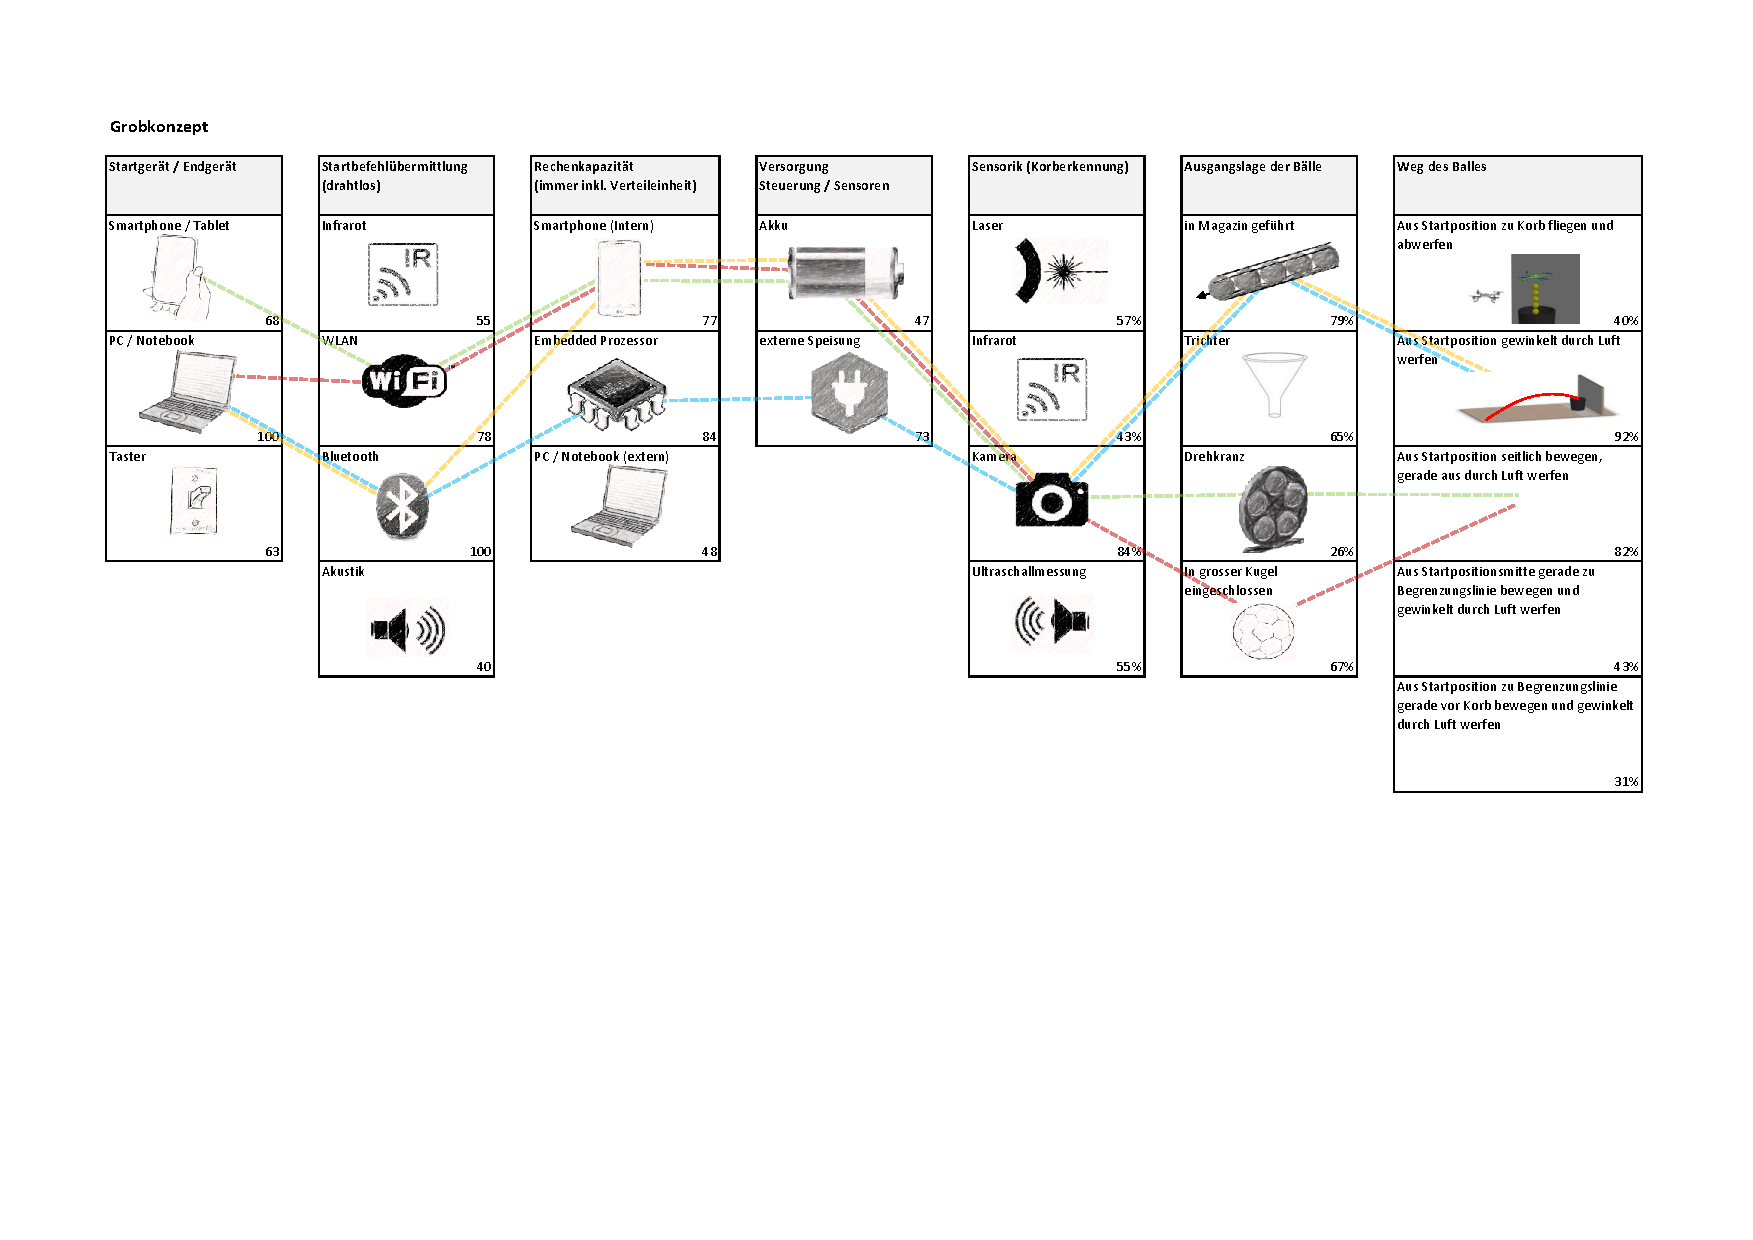
\includegraphics[page=1,scale=0.75,clip,trim=17mm 37mm 21mm 19mm]{Morphologie/Bilder/Grobkonzept.pdf}
			\centering
			\caption{Grobkonzept} 
			\label{abb:Grobkonzept}
		\end{figure}	
\end{landscape} 

\parindent0pt{\textit{Die detaillierte Bewertung aller Varianten sind dem Anhang \ref{apx:BewertungGrobkonzepte} zu entnehmen.}}\\
\\
Es wurden vier Varianten (orange, grün, rot, blau), wie in Abbildung \ref{abb:Grobkonzept} ersichtlich, gewählt. 
\begin{itemize}
	\item Blaue Variante\\
	Eine Auswahl aller Lösungen, welche die höchste Punktezahl durch die Bewertungskriterien erreichte.
	
	\item Rote Variante\\
	Ausgangspunkt in dieser Variante ist die Auswahl, die Bälle in eine Kugel einzuschliessen. Da ein Smartphone mit integrierter Kamera verwendet wird, kann man zwei Teilprobleme mit einem Gerät lösen. Den Weg des Balles via seitliche Verschiebung wurde aufgrund der Unhandlichkeit der grossen Kugel gewählt: der Weg soll kurz und einfach gehalten werden. Der Akku dient in dieser Variante neben der Energieversorgung auch als Ballast, um dem grossen Gewicht der Kugel entgegenzuwirken. Weiter ist die Ausgabe des Startsignals mit einem Notebook, sowie die Übertragung mit WLAN leicht zu Realisieren, da diese Lösungen auf gut dokumentierten Technologien basieren.
	
	\item Grüne Variante\\
	Für die grüne Variante wurde als Ausgangslage der Bälle die Führung in einem Drehkranz gewählt. Kongruent zur Variante Rot, wurde auch hier der Weg des Balles via seitliche Verschiebung aufgrund der Unhandlichkeit des Drehkranzes als Favorit erkoren. Für die Wahl des Akkus, der Startsignal-Übertragung per WLAN und die Verwendung eines Smartphones überzeugten dieselben Kriterien, welche bereits in der roten Variante genannt wurden.
	
	\item Orange Variante\\
	Aus der Startposition gewinkelt werfen, ist der Ursprung der orangen Variante. Eine geführte Ausgabe aus einem Magazin hat den Vorteil, dass es mit leichten Materialen gebaut werden kann, verschiedene Formen, Winkel und Ausgabegeschwindigkeiten zur Verfügung stehen. Der Akku dient in dieser Variante neben der Energieversorgung auch als Ballast und hat den schönen Nebeneffekt, dass das System energieautark ist.
\end{itemize}

\subsection{Entscheidung}
Die orange Variante bietet als gesamtes Konzept die erfolgversprechendste und effizienteste Lösung, bezüglich der vordefinierten Ziele der Team-Charta. Den Ball von der Startposition aus gewinkelt durch die Luft zu werfen erfordert keine zusätzlichen Bauteile um das Produkt am Boden zu verschieben. Dies minimiert einerseits den Aufwand und verringert die Fehleranfälligkeit erheblich. Die Bälle in der Ausgangslage in einem Magazin zu führen hat den Vorteil, dass eine allfällige stückweise Ausgabe der Bälle mit wenig Aufwand hinzugefügt werden kann. Ein Smartphone mit integrierter Kamera löst die zwei Teilprobleme der Korberkennung und Rechenkapazität mit einem Gerät. Des weiteren wäre das Produkt durch die Verwedung eines Akkus energieautark. Die Ausgabe des Startsignals und Endsignals mit einem Notebook und die Übermittlung mit Bluetooth sind einfach auszuführen und beruhen auf wohlbekannten, gut dokumentierten Technologien.
    
    %\newcommand{\myspace}{3.1cm}

\section{(Erklärung)}
	Um ein Grobkonzept erstellen zu können, wurde die Aufgabe in Teilprobleme unterteilt. Diese wurden anschliessend einem Brainstorming-Prozess unterworfen. Aus den daraus resultierten Ideen wurde ein Morphologischer Kasten erstellt und gewichtet.
\begin{landscape}
	\section{Morphologische Kästen}
	
	\begin{tabular}{|p{\myspace}|p{\myspace}|p{\myspace}|p{\myspace}|p{\myspace}|p{\myspace}|} \hline
	\textbf{Ausgangslage der Bälle} & \textbf{Positions-ermittlung Korb} & \textbf{Transport der Bälle} & \textbf{Art des Transportes} & \textbf{Versorgungs-konzept} & \textbf{Steuerungs-konzept}\\ \hline
	
	Vereinzelte Ausgabe aus Magazin & Laservermessung & Aus Startposition zu Korb fliegen und abwerfen & Verworfene Bälle aufsammeln und erneut (ab)werfen & \cellcolor{green}Strom - Akku & Rechnen auf externem PC - einfacher Controller\\ \hline
	\cellcolor{green}Fortlaufende Ausgabe aus Magazin & Infrarotmessung & \cellcolor{green}Aus Startposition gewinkelt durch Luft werfen & Bälle auf einmal schiessen & Strom - extern & Embedded Prozessor auf Gerät \\ \hline
	Trichter & \cellcolor{green}Kamera & Aus Startposition, seitlich bewegen, gerade aus durch Luft werfen & \cellcolor{green}Bälle einzeln schiessen & Pneumatik & \cellcolor{green}Smartphone + Controller auf Gerät\\ \hline
	Drehkranz & Ultraschallmessung & Aus Startpositionmitte gerade zu Begrenzungslinie bewegen und gewinkelt durch Luft werfen & & Hydraulik & Smartphone extern + Controller auf Gerät\\ \hline
	In grosser Kugel eingeschlossen& Fliegender Messfühler & Aus Startposition zu Begrenzungslinie gerade vor Korb bewegen und durch Luft werfen & & mechanisch & \\ \hline
		
\end{tabular}
%	\begin{tabular}{|p{\myspace}|p{\myspace}|p{\myspace}|p{\myspace}|p{\myspace}|p{\myspace}|} \hline
%	\textbf{Ausgangslage der Bälle} & \textbf{Positions-ermittlung Korb} & \textbf{Transport der Bälle} & \textbf{Art des Transportes} & \textbf{Versorgungs-konzept} & \textbf{Steuerungs-konzept}\\ \hline
%	
%	Vereinzelte Ausgabe aus Magazin & Laservermessung & Aus Startposition zu Korb fliegen und abwerfen & Verworfene Bälle aufsammeln und erneut (ab)werfen & Strom - Akku & Rechnen auf externem PC - einfacher Controller\\ \hline
%	Fortlaufende Ausgabe aus Magazin & Infrarotmessung & Aus Startposition gewinkelt durch Luft werfen & Bälle auf einmal schiessen & Strom - extern & Embedded Prozessor auf Gerät \\ \hline
%	Trichter & Kamera & Aus Startposition, seitlich bewegen, gerade aus durch Luft werfen & Bälle einzeln schiessen & Pneumatik & Smartphone + Controller auf Gerät\\ \hline
%	Drehkranz & Ultraschallmessung & Aus Startpositionmitte gerade zu Begrenzungslinie bewegen und gewinkelt durch Luft werfen & & Hydraulik & Smartphone extern + Controller auf Gerät\\ \hline
%	In grosser Kugel eingeschlossen& Fliegender Messfühler & Aus Startposition zu Begrenzungslinie gerade vor Korb bewegen und durch Luft werfen & & mechanisch & \\ \hline
	
%	\end{tabular}
\end{landscape} 
    \appendix
    % Beginn des Anhangs
        \begin{appendix}
            \clearpage
            \pagenumbering{Roman} % römische Nummerierung des Anhangs (Grosse Buchstaben)
            \section{Anhang}
            %\newpage
            \subsection{Beurteilung}
\label{apx:Beurteilung}
            \newpage
        \end{appendix}  
\end{document}